\documentclass[10pt,letterpaper]{article}
\usepackage[lmargin=2.2in,rmargin=0.7in,
            tmargin=1.0in,bmargin=1.0in]{geometry}
\usepackage{notes}
\begin{document}

\begin{center}
\Large\textbf{3.4 -  Heaviside functions, Piece-wise Functions}\\
\normalsize (Section 3.1)
\end{center}

%%%%%%%%%%%%%%%%%%%%%%%%%%%%%%%%%%%%%%%%%%%%%%%%%%%%%%%%%%%
\section{Motivation for Discontinuous Functions}

\subsection{Modeling Delayed Effects}
Suppose a fish farm initially contains $100$ fish.
Without harvesting, the population grows according to
\[
P'=0.1P,\qquad P(0)=100,
\]
so the fish population is $P(t)=100e^{0.1t}$, where $t$ is measured in years. Now suppose we want to introduce a delayed effect into our model. Let's say after waiting five years, the farmers begin removing $30$ fish per year. We can model the fish population using a \textit{discontinuous function}:
\[
P'=0.1P+f(t),\qquad P(0)=100,
\]
where
\[
f(t)=
\begin{dcases}
0, & 0\le t<5,\\
-30, & t\ge5.
\end{dcases}
\]
\subsection{Delayed Harvesting}
The function $f(t)$ represents \textit{delayed harvesting}. Delayed harvesting introduces a shift in the dynamics at future time. Even when $f(t)$ is discontinuous the solution $P(t)$ is actually continuous as shown in the figure below. This makes logical sense because the fish are not magically vanishing; they're being farmed. We could solve this problem using undetermined coefficients separately before and after $t=5$, but we would like a method
that handles the entire problem at once.

\begin{figure}[H]
\centering
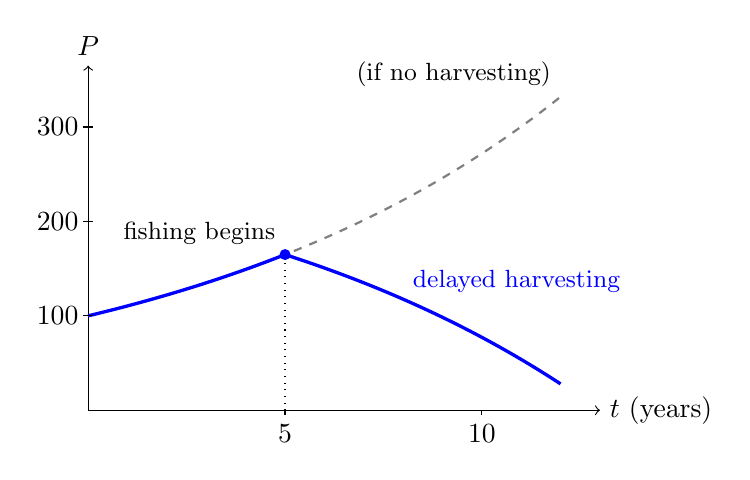
\begin{tikzpicture}[x=0.5cm,y=0.012cm]
    % Axes
    \draw[->] (0,0) -- (13,0)
        node[right] {$t$ (years)};
    \draw[->] (0,0) -- (0,365)
        node[above] {$P$};

    % No harvesting
    \draw[gray,dashed,thick,domain=0:12,samples=150]
        plot (\x,{100*exp(0.1*\x)});

    % Before harvesting
    \draw[blue,very thick,domain=0:5,samples=100]
        plot (\x,{100*exp(0.1*\x)});

    % After harvesting begins
    \draw[blue,very thick,domain=5:12,samples=150]
        plot (\x,{
            300+(100*exp(0.5)-300)*exp(0.1*(\x-5))
        });

    % Switching time
    \draw[dotted] (5,0) -- (5,{100*exp(0.5)});
    \fill[blue] (5,{100*exp(0.5)}) circle (2pt);
    \node[above left] at (5,{100*exp(0.5)})
        {\small fishing begins};

    % Tick labels
    \foreach \t in {5,10}{
        \draw (\t,0) -- (\t,-5);
        \node[below] at (\t,-5) {$\t$};
    }
    \foreach \p in {100,200,300}{
        \draw (-0.12,\p) -- (0.12,\p);
        \node[left] at (0,\p) {$\p$};
    }

    % Curve labels
    \node[above left] at (12,{100*exp(1.2)})
        {\small (if no harvesting)};
    \node[above right,blue] at (8,115)
        {\small delayed harvesting};
\end{tikzpicture}
\caption{The blue curve $P(t)$ represents the fish population over 12 years. Fish population is on an upward trend until $t=5$ when the harvesting begins.}
\end{figure}

\subsection{Goal}
More generally, our goal is to solve equations of the form
\[
ax''+bx'+cx=f(t),
\]
where the forcing term $f(t)$ is \textit{piecewise} and potentially \textit{discontinuous}.
Laplace transforms are particularly useful for these problems. However, we will not be solving this equation today. We will focus on how to find transforms and inverse transforms for piecewise functions.



%%%%%%%%%%%%%%%%%%%%%%%%%%%%%%%%%%%%%%%%%%%%%%%%%%%%%%%%%%%
\section{Heaviside Function and its Uses}

\subsection{Definition}

The \textbf{Heaviside function}, or \textbf{unit step function},
is defined by
\[
H(t)=
\begin{dcases}
0, & t<0,\\
1, & t\ge0.
\end{dcases}
\]
It is often useful to translate the Heaviside along the $t$-axis. For example, if we wanted to shift $H(t)$ to the right by $4$ units, we would write
\[
H(t-4)=
\begin{dcases}
0, & t-4<0,\\
1, & t-4\ge 0.
\end{dcases} \quad \implies \quad H(t-4) =\begin{dcases}
0, & t<4,\\
1, & t\ge 4.
\end{dcases} 
\]
Think of $H(t-4)$ as a switch that is initially turned off and then switches on at $t=4$. The sketches of $H(t)$ and $H(t-4)$ are plotted below. Use open and filled circles at the jumps to indicate the value of the function at the discontinuity.

\begin{figure}[H]
\centering
\begin{subfigure}[t]{0.47\linewidth}
\centering
\begin{tikzpicture}[x=1cm,y=1.1cm]
    \draw[->] (-1.2,0) -- (3.4,0) node[right] {$t$};
    \draw[->] (0,-0.25) -- (0,1.5) node[above] {$H$};

    \draw[red,very thick] (-1.1,0) -- (0,0);
    \draw[red,very thick] (0,1) -- (3.1,1);
    \draw[red,fill=white] (0,0) circle (2pt);
    \fill[red] (0,1) circle (2pt);

    \node[below right] at (0,0) {$0$};
    \node[left] at (0,1) {$1$};
\end{tikzpicture}
\caption{$H(t)$}
\end{subfigure}
\hfill
\begin{subfigure}[t]{0.47\linewidth}
\centering
\begin{tikzpicture}[x=1cm,y=1.1cm]
    \draw[->] (-1.2,0) -- (3.4,0) node[right] {$t$};
    \draw[->] (0,-0.25) -- (0,1.5) node[above] {$H$};

    \draw[red,very thick] (-1.1,0) -- (1.5,0);
    \draw[red,very thick] (1.5,1) -- (3.1,1);
    \draw[red,fill=white] (1.5,0) circle (2pt);
    \fill[red] (1.5,1) circle (2pt);

    \node[below] at (1.5,0) {$t=4$};
    \node[left] at (0,1) {$1$};
\end{tikzpicture}
\caption{$H(t-4)$}
\end{subfigure}
\caption{The shift $4$ controls the time at which the jump occurs.}
\end{figure}
Using this simple function, we may construct an \textbf{in-line representation} of piecewise functions. For example, the delayed harvesting function
$$
f(t)=
\begin{dcases}
0, & 0\le t<5,\\
-30, & t\ge5.
\end{dcases}
$$
can be written in one line as $f(t)=-30H(t-5).$


%-------------------------------------------------------------
\subsection{Suppressing vs. Delaying}

Suppose $f(t)$ models an external force. This may be the forcing function for a differential equation. Multiplying a function $f(t)$ by a Heaviside function has some interesting properties. 
\begin{enumerate}
\item Multiplying $f(t)$ by $H(t-a)$ yields
\[
f(t)H(t-a)=
\begin{dcases}
0, & t<a,\\
f(t), & t\ge a.
\end{dcases}
\]
The product is zero until time $t=a$. This results in \textit{suppressing} the effect of $f(t)$ on a system until time $t=a$. 

\item Now suppose $f(t)$ changes with time. Multiplying $f(t-a)$ by $H(t-a)$ yields
\[
f(t-a)H(t-a)=
\begin{dcases}
0, & t<a,\\
f(t-a), & t\ge a.
\end{dcases}
\]
At $t=a$, the delayed function begins with the value $f(0)$. This results in \textit{delaying} the start of $f(t)$ until time $t=a$. 
\end{enumerate}
The following example illustrates the graphical difference between the two effects.

\begin{example}[1]{
Let $f(t)=t$. Sketch and compare
\[
tH(t-2)
\qquad\text{and}\qquad
(t-2)H(t-2).
\]
}
Write each function piecewise:
\[
tH(t-2)=
\begin{dcases}
0, & t<2,\\
t, & t\ge2,
\end{dcases}
\qquad
(t-2)H(t-2)=
\begin{dcases}
0, & t<2,\\
t-2, & t\ge2.
\end{dcases}
\]
The first function switches on at height $2$.
The second starts at height $0$ and follows the original
ramp with a delay of two units.

\begin{center}
\begin{minipage}[t]{0.47\linewidth}
\centering
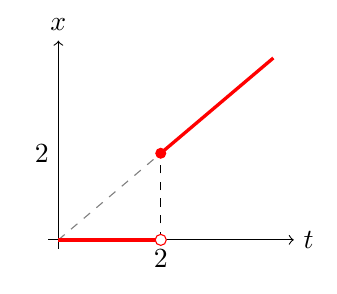
\begin{tikzpicture}[x=0.65cm,y=0.55cm]
    \path[use as bounding box]
        (-0.6,-0.6) rectangle (4.9,4.9);
    \draw[->] (-0.2,0) -- (4.6,0) node[right] {$t$};
    \draw[->] (0,-0.2) -- (0,4.6) node[above] {$x$};

    \draw[gray,dashed] (0,0) -- (2,2);
    \draw[red,very thick] (0,0) -- (2,0);
    \draw[red,very thick] (2,2) -- (4.2,4.2);
    \draw[dashed] (2,0) -- (2,2);
    \draw[red,fill=white] (2,0) circle (2pt);
    \fill[red] (2,2) circle (2pt);

    \node[below] at (2,0) {$2$};
    \node[left] at (0,2) {$2$};
\end{tikzpicture}

\small $tH(t-2)$
\end{minipage}
\hfill
\begin{minipage}[t]{0.47\linewidth}
\centering
\begin{tikzpicture}[x=0.65cm,y=0.55cm]
    \path[use as bounding box]
        (-0.6,-0.6) rectangle (4.9,4.9);
    \draw[->] (-0.2,0) -- (4.6,0) node[right] {$t$};
    \draw[->] (0,-0.2) -- (0,4.6) node[above] {$x$};

    \draw[red,very thick] (0,0) -- (2,0);
    \draw[red,very thick] (2,0) -- (4.2,2.2);
    \fill[red] (2,0) circle (2pt);

    \node[below] at (2,0) {$2$};
    \node[left] at (0,2) {$2$};
\end{tikzpicture}

\small $(t-2)H(t-2)$
\end{minipage}
\end{center}
\end{example}


\subsection{Jump from Constant to Constant}

Consider a function that jumps from one constant to another constant at time $t=a$. For example, 
$$
    f(t)  = \begin{dcases}
        L_1, & t<a\\
        L_2, & t\ge a.
    \end{dcases}
$$
This function can be written compactly in one line using the Heaviside function
\[
\boxed{
f(t)=L_1+(L_2-L_1)H(t-a).
}
\]
The function starts off at level $L_1$. Then at time $t=a$, the difference $L_2-L_1$ is added to simultaneously remove $L_1$ and introduce $L_2$.

\begin{example}[2]{
Sketch the function and write it using Heaviside functions:
\[
f(t)=
\begin{dcases}
3, & 0\le t<2,\\
5, & 2\le t<3,\\
-1, & t\ge3,\\
\end{dcases}
\]
}
Start at $3$. The successive changes are
\[
\begin{array}{c|c|c}
\text{Time} & \text{Change in value} & \text{Term to add}\\
\hline
0 & 3 & \\
2 & 5-3=2  & 2H(t-2)\\
3 & -1-5=-6 & -6H(t-3)\\
\end{array}
\]
Therefore, $f(t)$ can be written as 
\[
\boxed{
f(t)=3+2H(t-2)-6H(t-3).
}
\]

\begin{center}
\begin{tikzpicture}[x=0.9cm,y=0.5cm]
    % Axes
    \draw[->] (-0.3,0) -- (6,0) node[right] {$t$};
    \draw[->] (0,-1.8) -- (0,6) node[above] {$f(t)$};

    % Function
    \draw[red,very thick] (0,3) -- (2,3);
    \draw[red,very thick] (2,5) -- (3,5);
    \draw[red,very thick,->] (3,-1) -- (5.7,-1);

    % Included endpoints
    \foreach \x/\y in {0/3,2/5,3/-1}
        \fill[red] (\x,\y) circle (2.5pt);

    % Excluded endpoints
    \foreach \x/\y in {2/3,3/5}
        \draw[red,fill=white,thick]
            (\x,\y) circle (2.5pt);

    % Axis labels
    \foreach \x in {2,3}{
        \draw (\x,-0.1) -- (\x,0.1);
        \node[below] at (\x,0) {$\x$};
    }
    \foreach \y in {-1,3,5}{
        \draw (-0.08,\y) -- (0.08,\y);
        \node[left] at (0,\y) {$\y$};
    }
\end{tikzpicture}
\end{center}

\end{example}

%-------------------------------------------------------------
\subsection{Jump from Function to Function}

The same method works when the pieces are functions:
\[
f(t)=
\begin{dcases}
g(t), & 0\le t<a,\\
h(t), & t\ge a.
\end{dcases}
\]
Start with $g(t)$, then at $t=a$ simultaneously add $h(t)$ and subtract $g(t)$:
\[
\boxed{
f(t)=g(t)+\bigl(h(t)-g(t)\bigr)H(t-a).
}
\]
Before $a$, the added term is zero. After $a$, the
expression simplifies to $g(t)+h(t)-g(t)=h(t)$.

\begin{example}[3]{
Write the following function using a Heaviside function:
\[
f(t)=
\begin{dcases}
1, & 0\le t<1,\\
t^2, & t\ge1.
\end{dcases}
\]
}
The initial expression is $1$, and the new expression
is $t^2$. Thus,
\[
\boxed{f(t)=1+(t^2-1)H(t-1).}
\]
\end{example}

%%%%%%%%%%%%%%%%%%%%%%%%%%%%%%%%%%%%%%%%%%%%%%%%%%%%%%%%%%%%%%%%%%%%%%%%
\section{Transform Formulas}

\subsection{Transform of the Heaviside Function}
Here is the first transform formula involving the step functions. For $a\ge0$,
\[
\boxed{
\mathcal L[H(t-a)]=\frac{e^{-as}}{s},
\qquad s>0.
}
\]
This is formula number 8 in the Laplace table.
The proof of this formula will be a homework exercise.
% \begin{proof}
% The step function is zero before $a$ and one afterward:
% \begin{align*}
% \mathcal L[H(t-a)]
% &=\int_0^\infty H(t-a)e^{-st}\,dt\\
% &=\int_a^\infty e^{-st}\,dt
% &&\com{$H=0$ before $a$, $H=1$ after $a$}\\
% &=\lim_{R\to\infty}
%   \left[-\frac{e^{-st}}{s}\right]_a^R\\
% &=\lim_{R\to\infty}
%   \frac{e^{-as}-e^{-Rs}}{s}\\
% &=\frac{e^{-as}}{s},
% &&\com{$s>0$}
% \end{align*}
% as claimed.
% \end{proof}
This formula allows us to find transforms of some piecewise functions. Take the harvesting function, for example 
\[
f(t)=
\begin{dcases}
0, & 0\le t<5,\\
-30, & t\ge5.
\end{dcases}
\]
To find the transform of $f(t)$, you must first rewrite it using the step function
$$
    f(t)=-30H(t-5).
$$
Then we can apply the new formula 
$$
    \mathcal{L}\left[f(t)\right] = \mathcal{L}\left[-30H(t-5)\right] = -30 \frac{e^{-5s}}{s}. 
$$


%-------------------------------------------------------------
\subsection{Transform of a Delayed Function}

The product $H(t-a)f(t-a)$ has the effect of delaying the start of $f(t)$ until $t=a$. There is a formula for the transform of this product. Let $\mathcal L[f(t)]=F(s)$ and $a\ge0$. Then
\[
\boxed{
\mathcal L[H(t-a)f(t-a)]=e^{-as}F(s).
}
\]
This is formula 9a in the Laplace table. The textbook calls this the \textbf{switching property}. The proof of this formula is left as a homework exercise.
% \begin{proof}
% Begin with the definition and substitute $u=t-a$:
% \begin{align*}
% \mathcal L[H(t-a)f(t-a)]
% &=\int_a^\infty f(t-a)e^{-st}\,dt\\
% &=\int_0^\infty f(u)e^{-s(u+a)}\,du
% &&\com{$u=t-a$, so $t=u+a$}\\
% &=e^{-as}\int_0^\infty f(u)e^{-su}\,du\\
% &=e^{-as}F(s).
% \end{align*}
% \end{proof}
Here is an example of how to utilize this formula.

\begin{example}[4]{
Find the transform
\[
\mathcal L[(t-3)^2H(t-3)].
\]
}
\paragraph{Step 1.} Write down the formula.
\[
\mathcal L[(t-3)^2H(t-3)] =\mathcal{L}\left[H(t-a)f(t-a)\right] =e^{-as}F(s).
\]
\paragraph{Step 2.} Identify the shift $a$ and the base transform. By comparison, 
\begin{align*}    
\mathcal L[H(t-3)(t-3)^2] &=\mathcal{L}\left[H(t-a)f(t-a)\right]
\end{align*}
we see that the shift is $a=3$ and the base transform is
\[
f(t)=t^2,
\qquad
F(s)=\mathcal L[t^2]=\frac{2}{s^3}.
\]
\paragraph{Step 3.} Substitute.
\[
\mathcal L[(t-3)^2H(t-3)] =e^{-as}F(s)
=e^{-3s}F(s)
=\boxed{\frac{2e^{-3s}}{s^3}.}
\]
\end{example}
%-------------------------------------------------------------
\subsection{When Shifts Do Not Match}
In the previous example, 
\[
 x(t)=\underbrace{(t-3)^2}_{\text{shift 3}}\underbrace{H(t-3)}_{\text{shift 3}}
\]
the shifts matched. In some functions, such as 
$$
x(t)=\underbrace{e^{3t}}_{\text{shift 0}}\underbrace{H(t-2)}_{\text{shift 2}} 
$$
the shifts do not match. There are two options to deal with this:
\paragraph{Option 1:} Rewrite the exponential so that
its shift matches the step function:
\begin{align*}
e^{3t}H(t-2)
&=e^{3(t-2+2)}H(t-2)\\
&=e^6e^{3(t-2)}H(t-2).
\end{align*}
The base function is $f(t)=e^{3t}$, with transform
$F(s)=1/(s-3)$. Applying the switching property,
\begin{align*}
\mathcal L[e^{3t}H(t-2)]
&=e^6e^{-2s}\mathcal L[e^{3t}]\\
&=\boxed{\frac{e^{-2s+6}}{s-3}.}
\end{align*}
\paragraph{Option 2:} Since this occurs frequently, you can use this convenient formula 
\[
\boxed{
\mathcal L[f(t)H(t-a)]
=e^{-as}\mathcal L[f(t+a)]
}
\]
This is formula 9b in the Laplace table. The following example demonstrates how this works.

\begin{example}[5]{
Find
\[
\mathcal L[e^{3t}H(t-2)].
\]
}
Here, $f(t)=e^{3t}$ and $a=2$. Using formula 9b,
\begin{align*}
\mathcal L[e^{3t}H(t-2)]
&=e^{-2s}\mathcal L[e^{3(t+2)}]\\
&=e^{-2s}e^6\mathcal L[e^{3t}]\\
&=\boxed{\frac{e^{-2s+6}}{s-3}.}
\end{align*}
\end{example}

% \begin{example}[6]{
% Find the Laplace transform of the function from Example 3:
% \[
% f(t)=
% \begin{dcases}
% 1, & 0\le t<1,\\
% t^2, & t\ge1.
% \end{dcases}
% \]
% }
% We already wrote
% \[
% f(t)=1+(t^2-1)H(t-1).
% \]
% Apply linearity and the shortcut with $a=1$:
% \begin{align*}
% \mathcal L[f(t)]
% &=\frac1s+e^{-s}\mathcal L[(t+1)^2-1]\\
% &=\frac1s+e^{-s}\mathcal L[t^2+2t]\\
% &=\boxed{
% \frac1s+e^{-s}\left(\frac2{s^3}+\frac2{s^2}\right).
% }
% \end{align*}
% Be sure to replace every $t$ in the switched expression
% by $t+a$ before taking its transform.
% \end{example}

%%%%%%%%%%%%%%%%%%%%%%%%%%%%%%%%%%%%%%%%%%%%%%%%%%%%%%%%%%%%%%%%%%%%%%%%
\section{Inverse Transforms}

\subsection{Switching Property in Reverse}
Since the goal is to solve differential equations with Heaviside forcing, we must learn how to  use the switching property in reverse. 
The inverse form of the switching property is
\[
\boxed{
\mathcal L^{-1}[e^{-as}F(s)]
=H(t-a)f(t-a)
}
\]
Use the following steps:
\begin{enumerate}
    \item Write the formula.
    \item Identify the shift $a$ and the base transform $f(t) \to F(s)$.
    \item Substitute
\end{enumerate}
The result is zero before the delay and follows
$f(t-a)$ afterward.

\begin{example}[6]{
Find the inverse transform and write the answer piecewise:
\[
\mathcal L^{-1}\left[
e^{-2s}\frac{2}{s^2+49}
\right].
\]
}
\paragraph{Step 1.} Write down the formula.
\[
\mathcal L^{-1}\left[
e^{-2s}\frac{2}{s^2+49}
\right]=\mathcal L^{-1}[e^{-as}F(s)]
=H(t-a)f(t-a).
\]
\paragraph{Step 2.} Identify the delay $a$ and the
base function. By comparison,
\[
a=2,\qquad F(s)=\frac{2}{s^2+49}\quad \implies\quad  f(t)=\mathcal L^{-1}\left[\frac{7}{7}\frac{2}{s^2+49}\right]
=\frac{2}{7}\sin7t.
\]
\paragraph{Step 3.} Substitute.
\[
x(t)=H(t-2)f(t-2)
=\boxed{\frac{2}{7}\sin(7(t-2))H(t-2).}
\]
% Replacing every $t$ in $f(t)$ by $t-2$ changes $\cos3t$ into $\cos(3(t-2))$. 
% In piecewise form,
% \[
% x(t)=
% \begin{dcases}
% 0, & 0\le t<2,\\
% 2\cos(3(t-2)), & t\ge2.
% \end{dcases}
% \]
\end{example}

%------------------------------------------------------
\subsection{Heaviside to Piecewise}
The advantage of Heaviside notation is its compactness. The solution to Example 6 can be written in a single line
$$
    x(t) = \frac{2}{7}\sin(7(t-2))H(t-2).
$$
But this can also be a downside since it is difficult to interpret. The function is easier to conceptualize when rewritten as a piecewise function: 
\[
x(t)=
\begin{dcases}
0, & 0\le t<2,\\
\frac{2}{7}\sin(7(t-2)), & t\ge2.
\end{dcases}
\]

\subsection{Moving Forward}
You are now ready to solve the IVP
\[
P'=0.1P+f(t),\qquad P(0)=100,
\]
where
\[
f(t)=
\begin{dcases}
0, & 0\le t<5,\\
-30, & t\ge5.
\end{dcases}
\]
We will do this in the next lecture. Naturally, we solve this equation with Laplace transforms. However, the solution $P(t)$ will be in terms of the Heaviside function. You will change it to piecewise form for interpretation.

% \subsection{Combining with Partial Fractions}

% Sometimes we must simplify $F(s)$ before finding
% the base function. The factor $e^{-as}$ stays outside
% while we do the partial fraction decomposition.

% \begin{example}[8]{
% Find the inverse transform and write the answer piecewise:
% \[
% \mathcal L^{-1}\left[
% \frac{e^{-3s}}{s(s+1)}
% \right].
% \]
% }
% \paragraph{Step 1.} Write down the formula.
% \[
% \mathcal L^{-1}[e^{-as}F(s)]
% =H(t-a)f(t-a).
% \]

% \paragraph{Step 2.} Identify the delay $a$ and the
% base function. By comparison,
% \[
% a=3,\qquad F(s)=\frac1{s(s+1)}.
% \]
% Use partial fractions to find the base function:
% \[
% F(s)=\frac1s-\frac1{s+1}
% \quad\implies\quad
% f(t)=1-e^{-t}.
% \]

% \paragraph{Step 3.} Substitute.
% \[
% x(t)=H(t-3)f(t-3)
% =\boxed{\bigl(1-e^{-(t-3)}\bigr)H(t-3).}
% \]
% In piecewise form,
% \[
% x(t)=
% \begin{dcases}
% 0, & 0\le t<3,\\
% 1-e^{-(t-3)}, & t\ge3.
% \end{dcases}
% \]
% \end{example}
%-------------------------------------------------------------
% \subsection{Combining Delayed and Undelayed Terms}

% Apply the inverse transform separately to each term.
% Only terms with an exponential factor $e^{-as}$
% receive a delay.

% \begin{example}[9]{
% Find the inverse transform and write the answer piecewise:
% \[
% X(s)=\frac1{s^2}-\frac{e^{-3s}}{s^2}.
% \]
% }
% Both rational parts have base function $f(t)=t$,
% but only the second term is delayed:
% \[
% \boxed{x(t)=t-(t-3)H(t-3).}
% \]
% Before $t=3$, the second term is off.
% After $t=3$, the expression becomes $t-(t-3)=3$.
% Therefore,
% \[
% x(t)=
% \begin{dcases}
% t, & 0\le t<3,\\
% 3, & t\ge3.
% \end{dcases}
% \]
% The graph rises linearly and then levels off.

% \begin{center}
% \begin{tikzpicture}[x=0.75cm,y=0.6cm]
%     \draw[->] (-0.2,0) -- (6.4,0) node[right] {$t$};
%     \draw[->] (0,-0.2) -- (0,3.9) node[above] {$x$};

%     \draw[red,very thick] (0,0) -- (3,3) -- (6,3);
%     \draw[dashed] (3,0) -- (3,3);

%     \fill[red] (3,3) circle (2pt);
%     \node[below] at (3,0) {$3$};
%     \node[left] at (0,3) {$3$};
% \end{tikzpicture}
% \end{center}
% \end{example}

% %%%%%%%%%%%%%%%%%%%%%%%%%%%%%%%%%%%%%%%%%%%%%%%%%%%%%%%%%%%%%%%%%%%%%%%%
% \section{Summary}

% The Heaviside function describes when an expression
% becomes active. The main switching property is
% \[
% \boxed{
% \mathcal L[H(t-a)f(t-a)]=e^{-as}F(s).
% }
% \]
% Read it backward to find inverse transforms:
% \[
% \boxed{
% \mathcal L^{-1}[e^{-as}F(s)]
% =H(t-a)f(t-a).
% }
% \]
% When the function has not been shifted, use
% \[
% \mathcal L[f(t)H(t-a)]
% =e^{-as}\mathcal L[f(t+a)].
% \]

% Do not confuse this with the exponential shift
% property from the previous lecture:
% \[
% \begin{array}{c|c}
% \text{Time domain} & \text{Laplace domain}\\
% \hline
% e^{at}f(t) & F(s-a)\\[2pt]
% H(t-a)f(t-a) & e^{-as}F(s)
% \end{array}
% \]
% Multiplication by an exponential shifts $s$.
% Delaying a function introduces an exponential factor
% in $s$.

% In the next lecture, we will use these formulas to
% solve IVPs with piecewise forcing.

\end{document}